\documentclass[UTF8]{ctexart} %使用ctex包,中文支持
\usepackage{amsmath}  %数学公式
\usepackage{graphicx} %插图
\usepackage{fancyhdr} %个性化页眉页脚
\usepackage{geometry} %页边距
\usepackage{bm}  % 公式加粗
\usepackage{float} %为了在分栏下插入图片
\usepackage{ulem}  % 换行下划线
%\usepackage{setspace} %行间距
\usepackage{multicol} %用于实现在同一页中实现不同的分栏
\geometry{a4paper,left=2cm,right=2cm,top=2cm,bottom=2cm} % 页边距设置

\title{集成学习笔记}
\author{宋佳欢}
\pagestyle{plain}

\begin{document}
	\maketitle
	\tableofcontents
	\songti \zihao{-4}
	
	\section{Bagging}
		什么情况适合做Bagging:模型容易过拟合(很强的模型),降低模型预测的方差。Bagging并不能帮助模型更好地拟合训练数据。
		\subsection{随机森林}
		决策树在训练数据上很容易达到0错误率(每个叶节点只包含一个样本)。随机森林时决策树的Bagging算法,两种实现方式:
		
		1.在m个样本的数据集D中,有放回地随机采样m个样本,将其拷贝进$D_1$。$D_1$中会有重复的样本,且部分D中的样本没有在$D_1$中出现。重复上述过程,得到n个不同的数据集${D_1,D_2,\cdots,D_n}$,用这些数据集分别训练n个决策树,构成随机森林。
		
		2.随机地限制某些特征在生成决策树时禁用,这样也能得到若干不同的决策树。
		
		out-of-bag validation for Bagging:
		若方法1训练决策树,可将那些在训练集中没有出现过的那些样本用于测试,这样就可以不用划分训练集和测试集了。
	\section{Boosting}
		什么情况适合做boosting:想要提升弱分类器的分类性能
		\begin{figure}[H]
			\centering{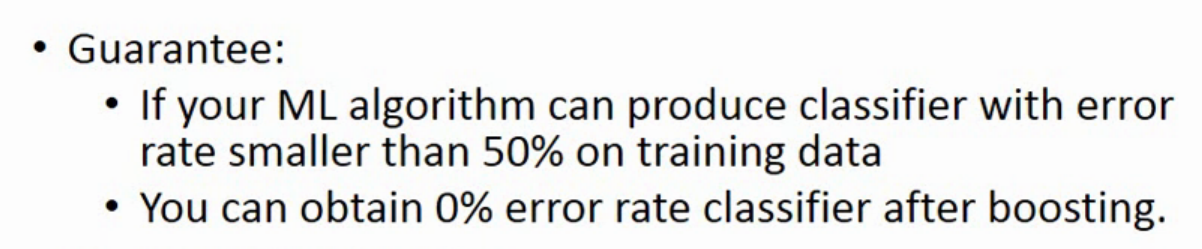
\includegraphics[scale=0.3]{1.png}}
		\end{figure}
		\subsection{Boosting的框架}
		
			1.得到一个弱分类器$f_1(x)$。
			
			2.找到另一个分类器$f_2(x)$取帮助$f_1(x)$。但是两者不能太相似,最好是互补的。
				
			3.同理,再找到另一个分类器$f_3(x)$取帮助$f_2(x)$。
			
			$\cdots$,最后结合所有的分类器。
			每个分类器都是按顺序学习的。
			
			为了获取不同的分类器,在不同的数据集上训练。为了得到不同的训练集,可以重采样来制造多个数据集;也可以为每个样本设置不同的权重,在实现中,只需在损失函数前为每个样本乘上一个权重即可:
			\[L(f)\sum_nl(f(x^n,\hat{y}^n))\Longrightarrow L(f)\sum_nu^nl(f(x^n,\hat{y}^n))\]
			其中$u^n$即为每个样本的权重。
		\subsection{Adaboost}
			主要思想:使用分类器$f_1(x)$分类失败的那些样本取训练$f_2(x)$。
			
			定义$f_1(x)$在训练集上的错误率为$\varepsilon_1$
			\[\varepsilon_1 = \frac{\sum_nu_1^n\delta(f_1(x^n)\neq\hat{y}^n)}{\sum_nu_1^n}\]
			$u_1^n$为训练第一个分类器时的第n个样本的权重。$\delta$函数括号内成立时等于1,否则等于0。若弱分类器由于随机分类,则有错误率$\varepsilon_1<0.5$。
			
			根据$u_1^n$调整$u_2^n$,即增大$f_1(x)$分类错误的样本的权重,减小分类正确的样本的权重,使得在训练$f_2(x)$时,分类器更加侧重于$f_1(x)$分类错误的样本的权重,使得两个分类器互相互补。调整权重使得$u_2^n$满足:
			\[\frac{\sum_nu_2^n\delta(f_1(x^n)\neq\hat{y}^n)}{\sum_nu_2^n}\]
			\begin{figure}[H]
				\centering{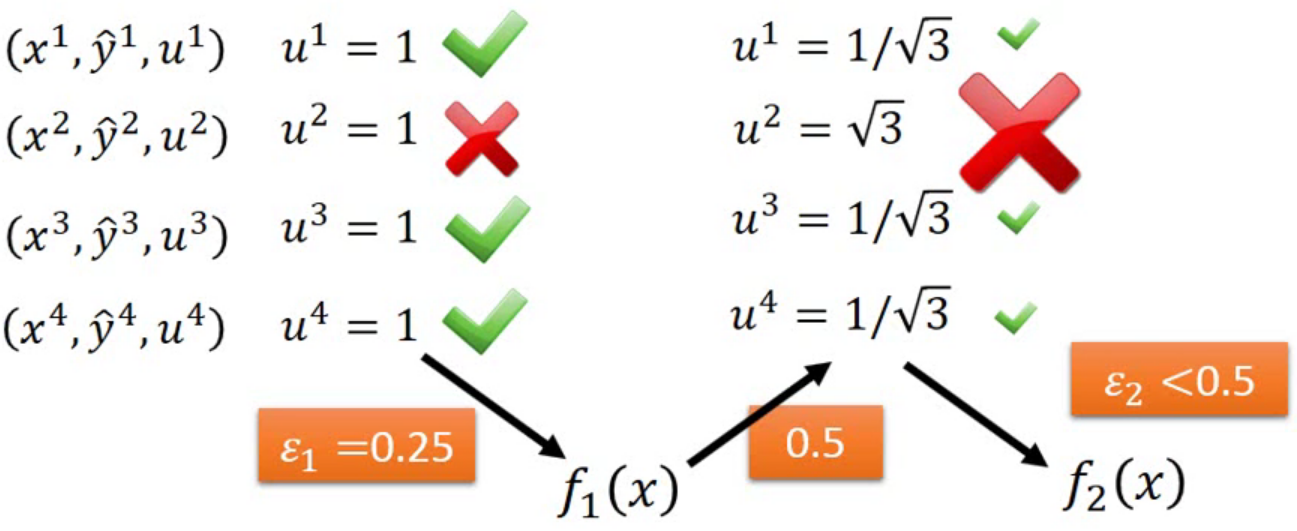
\includegraphics[scale=0.3]{2.png}}
			\end{figure}
			
			
			
			
			
			
		
\end{document}